\documentclass{beamer}
\usepackage{xcolor}
\usepackage{csquotes}
\usepackage{graphicx}
\usepackage{tasks}
% \usepackage[inline]{enumitem}

\definecolor{Violet}{RGB}{24,188,153}
\definecolor{VioletDark}{RGB}{14,147,119}

\title{GitHub}
\author{Edwin Kofler}
\hypersetup{
	colorlinks=true
}
\pdfinfo{
	/keywords (Git;GitHub)
}
\graphicspath{ {./assets} }
\settasks{style=enumerate}
% \subsectionfont{\color{astral}} % \sectionfont{\color{astral}}
% \useoutertheme{infolines}
\setbeamercolor{frametitle}{fg=VioletDark,bg=Violet!10}
\setbeamercolor{section in head/foot}{bg=Violet}
\setbeamercolor{author in head/foot}{bg=Violet}
\setbeamercolor{date in head/foot}{fg=Violet}

\begin{document}

% \frame{\titlepage}
\begin{frame}
	\titlepage
	\small{Links}
	\begin{tasks}[](4)
		\task \href{https://edwinkofler.com}{Website}
		\task \href{https://github.com/hyperupcall}{GitHub}
		\task \href{https://bsky.app/profile/hyperupcall.bsky.social}{Bluesky}
		\task \href{https://www.linkedin.com/in/hyperupcall}{LinkedIn}
	\end{tasks}
\end{frame}

\begin{frame}{Agenda}
	\begin{enumerate}
		\item Introduce Git
		\item Introduce GitHub
		\item Tour GitHub
		\item Using Other People's Repositories
	\end{enumerate}
\end{frame}

\begin{frame}{Introducing Git}
	From the official Git \href{https://git-scm.com}{website}: \newline

	\begin{displayquote}
		Git is a \href{https://git-scm.com/about/free-and-open-source}{free and open source} distributed version control system...
	\end{displayquote}

	{
	\small

	But what does that mean in practice? Git...

	\begin{itemize}
		\item Can record changes to files over time
		\item Can revert a project back to a previous state
		\item Track who last modified any particular file
	\end{itemize}
	}

	\href{https://raw.githubusercontent.com/ecc-cs-club/slides/main/1-Git-And-GitHub/assets/using-git.png}{
		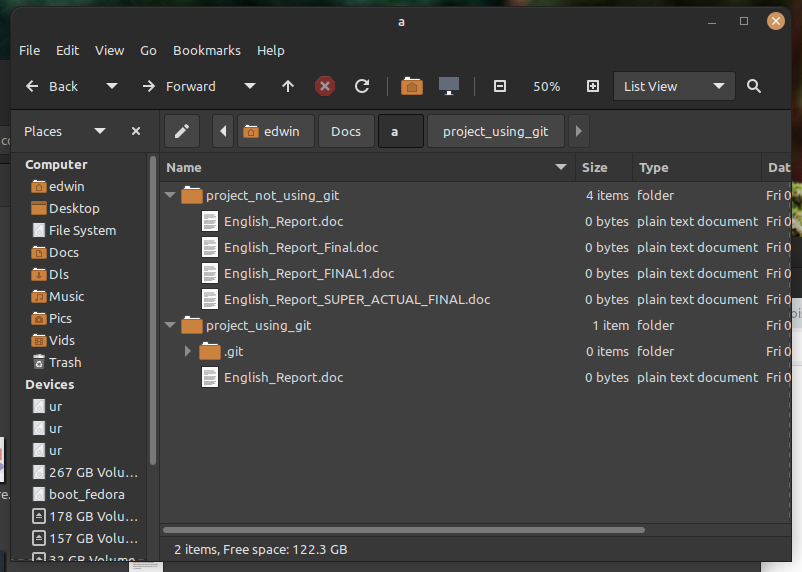
\includegraphics[width=6cm]{using-git.png}
	}


	\note{
		multiple people to work - if no git, would have to work on same computer. sometimes have trouble opening up files
		history - from a ``single file" to many many files like in those big projects
	}
\end{frame}

\begin{frame}{Git: Commits} \begin{itemize}
		\item Let's say we're working on a project called ``\textbf{Cool Project}"
		\item It might look like this, from the perspective of Git
	\end{itemize}
	\href{https://raw.githubusercontent.com/ecc-cs-club/slides/main/5-GitHub/assets/git-commit.png}{
		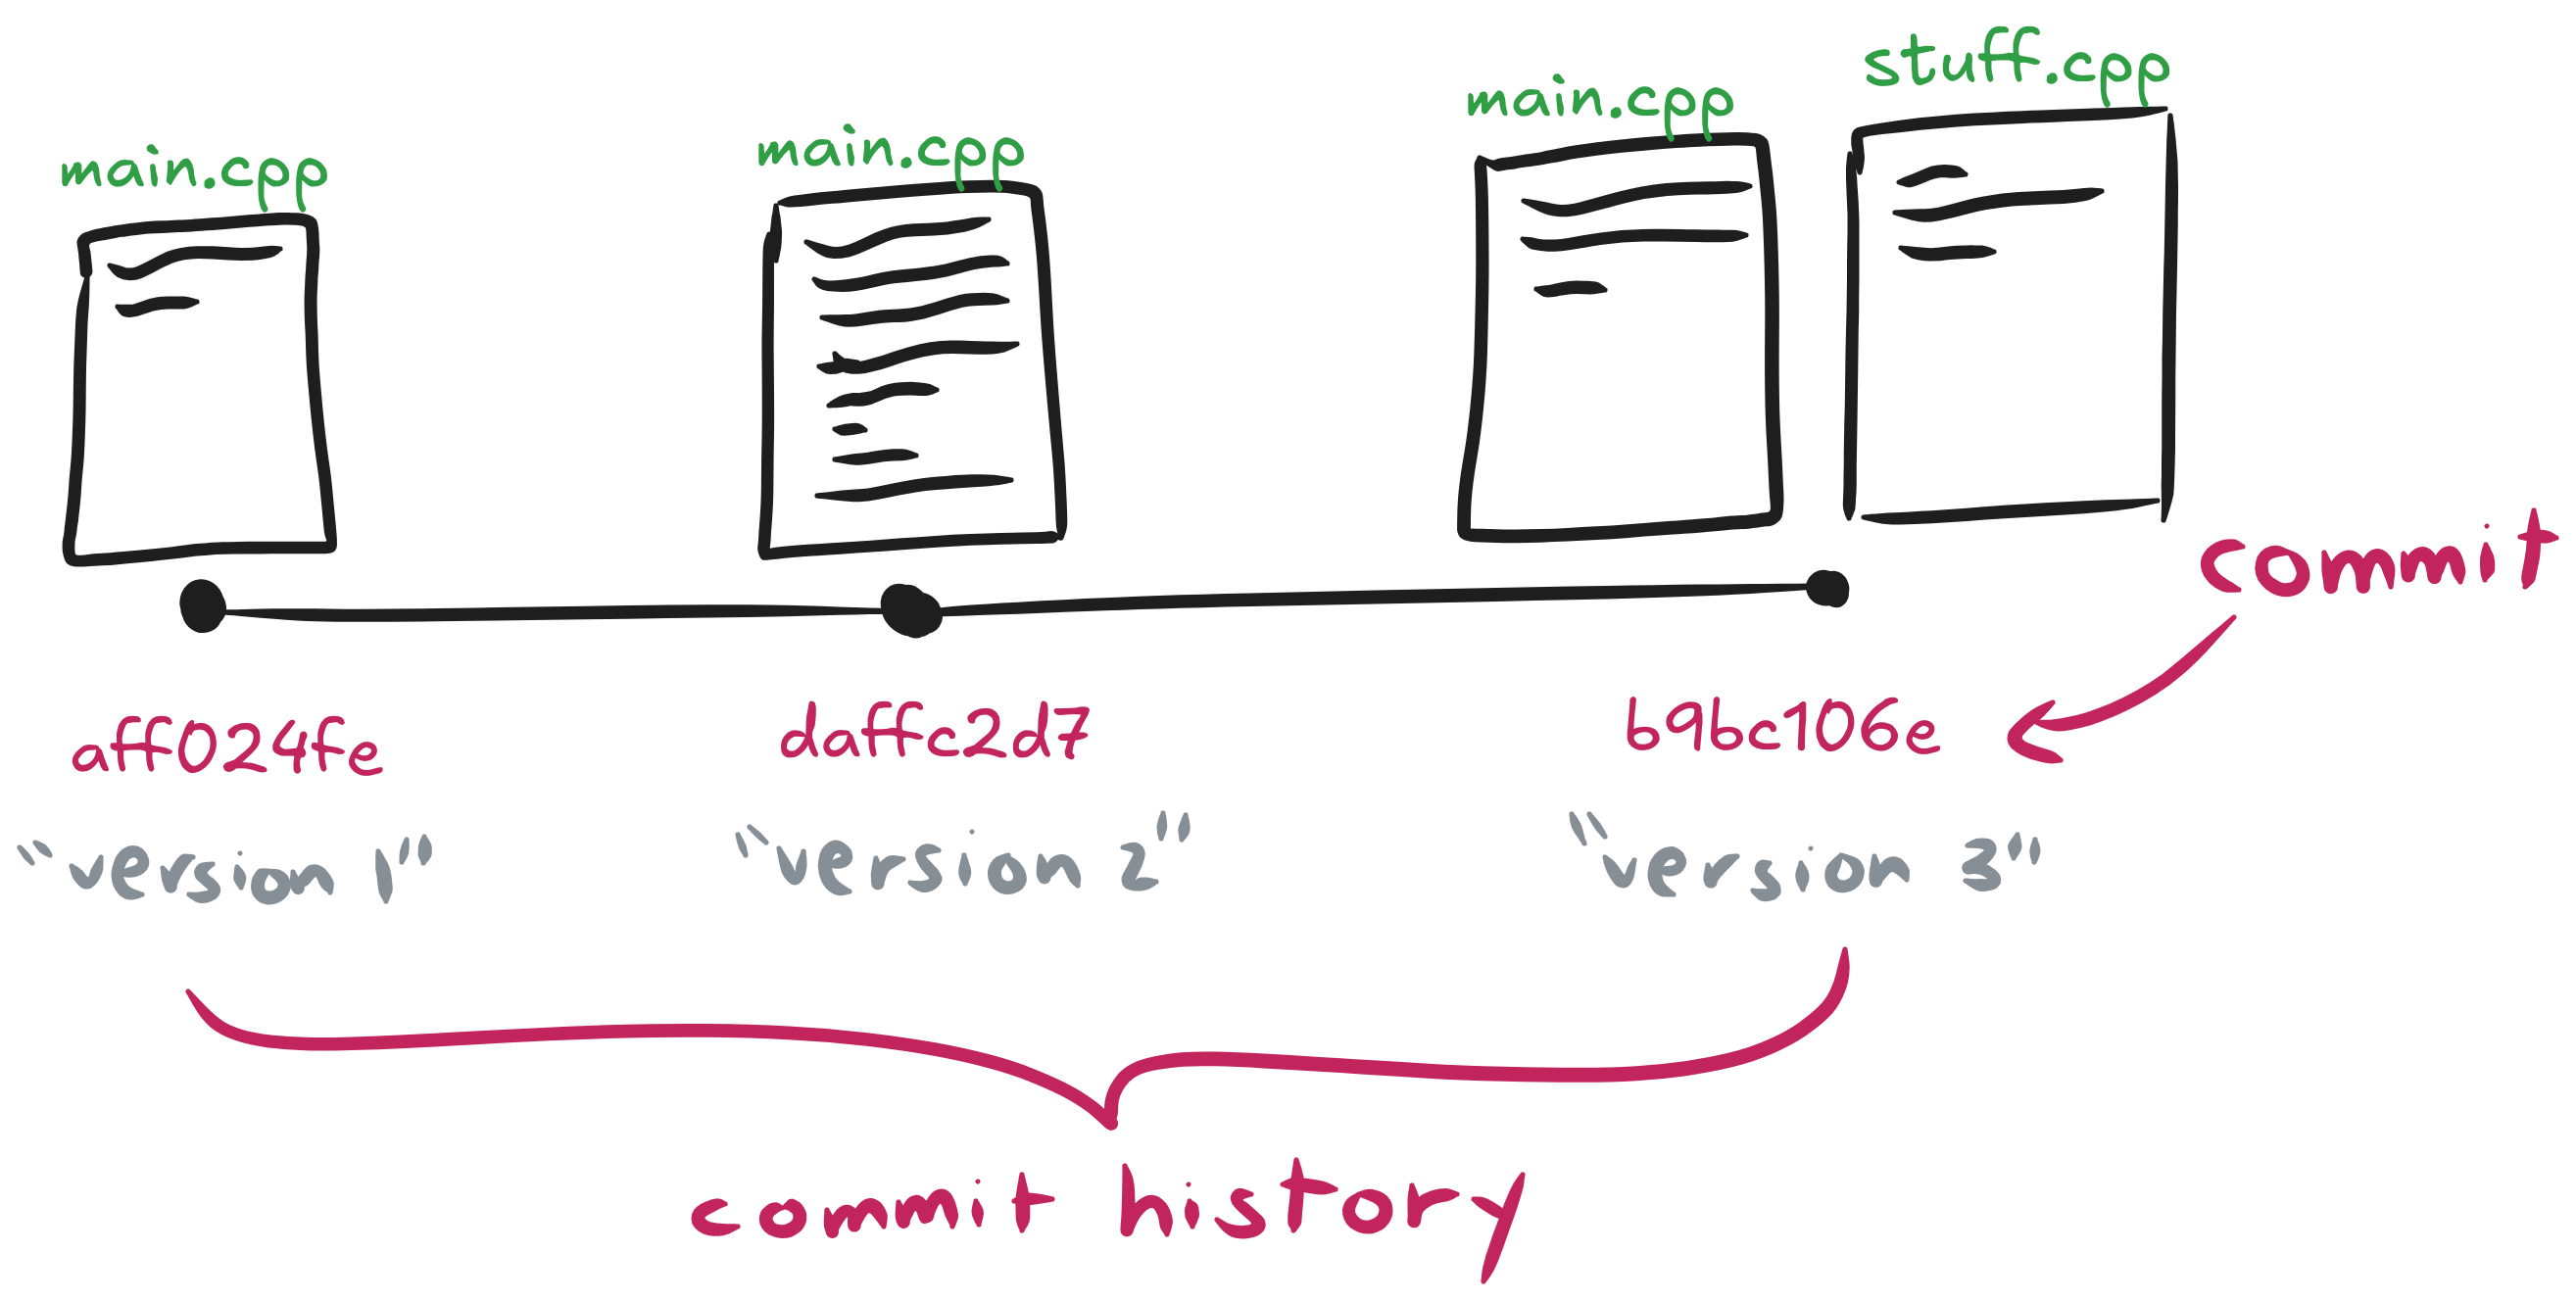
\includegraphics[width=11cm]{git-commit.png}
	}

	\note{
		- 1A. You wok on ``cool project'' for a while and finish 1st version
		- 1B. You tell git to ``add all my changes", and tell git to ``commit" or save my changes
		- Think of it like ``perfectly commiting something to memory''
		- 2A. And so on
		- Tie in with slide 1
		- Recording changes to files
		- Reverting a project back to previous state
	}
\end{frame}

\begin{frame}{Introducing GitHub}
	\begin{itemize}
		\item GitHub has a similar model to Dropbox
	\end{itemize}

	\href{https://raw.githubusercontent.com/ecc-cs-club/slides/main/5-GitHub/assets/github-dropbox.png}{
		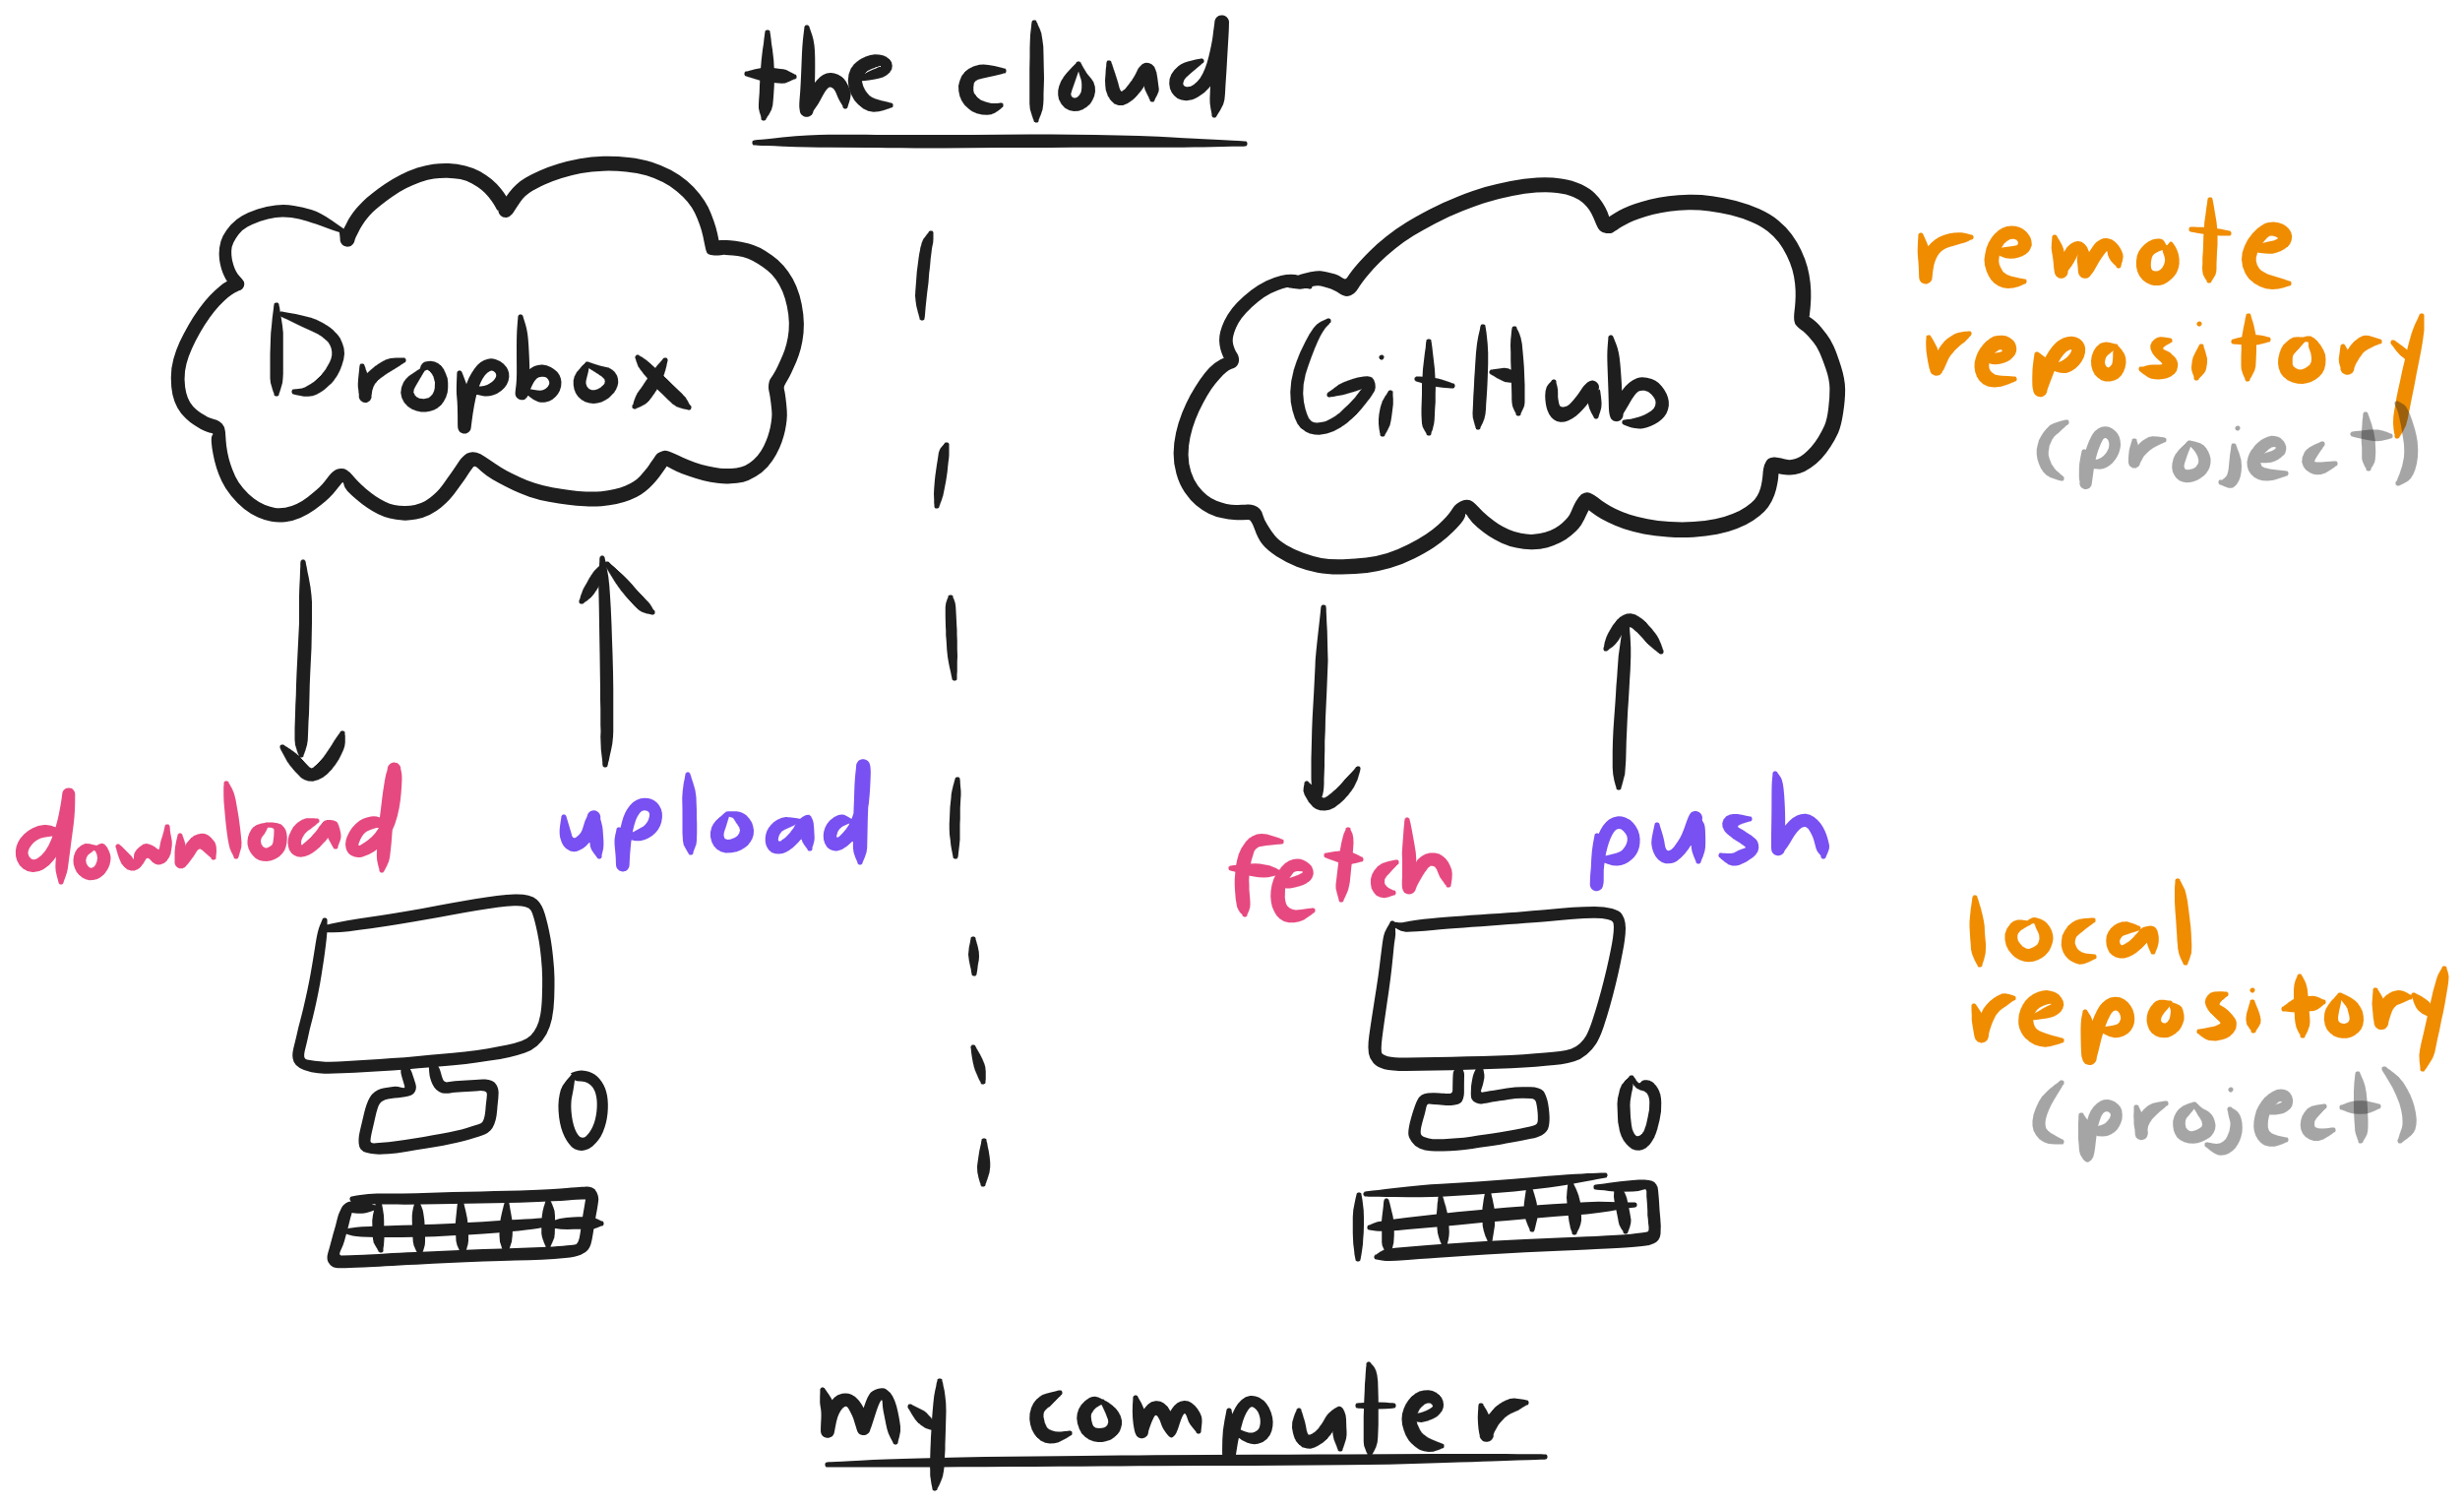
\includegraphics[width=10.5cm]{github-dropbox.png}
	}

	\note{
		Like Dropbox, sort of ``syncing" a folder on your computer with a remote server

		There is a \href{https://docs.github.com/en/get-started/signing-up-for-github/signing-up-for-a-new-github-account}{help page}, but it does not offer useful information
	}
\end{frame}

\begin{frame}{Tour of GitHub}
	\begin{itemize}
		\item Explore \href{https://github.com/fox-archives/demo-cool-project}{cool-project on GitHub}
		\item Create GitHub account
		\item Show ``profile" view
		\item Create/edit a ``profile README"
		\item Show large repository: \href{https://github.com/xournalpp/xournalpp}{xournalpp/xournalpp}
		      \begin{itemize}
			      \item {(See next slide)}
		      \end{itemize}
	\end{itemize}

	\vspace{0.25cm}
	{\large \textbf{Terms}}
	\begin{itemize}
		\item \textbf{repository:} a project that is tracked by Git
		\item \textbf{issue:} support ticket / a problem that needs to be solved
		\item \textbf{pull request:} updated/changed code that another person wants to add to the project
	\end{itemize}

	\note{
		- issues: open / closed / author filter
		- issues: scroll through some issues
		- issues ``good first issue" / ``sefault"
		- pull requests
		- pull requests: open / closed author filter
		- very often, issues correspond to pull requests
		- show pull requests
	}
\end{frame}

\begin{frame}{Using Other People's Repositories}
	This example / walkthrough requires the use of a GitHub account.

	\begin{itemize}
		\item 1. Fork the \texttt{cool-project} project (\only<1>{\href{https://docs.github.com/en/pull-requests/collaborating-with-pull-requests/working-with-forks/fork-a-repo\#forking-a-repository}{instructions here}})
		\item 2. Make sure you are on your personal/forked repository
		\item 3. Open project in github.dev (press ``." or replace ``github.com" with ``github.dev" in URL)
		\item In the \texttt{github.dev}, edit whatever code you want to edit
		\item Add, commit, and push your changes (\only<1>{\href{https://docs.github.com/en/codespaces/the-githubdev-web-based-editor\#commit-your-changes}{instructions here}})
		\item Make Pull Request? (\only<1>{\href{https://docs.github.com/en/codespaces/the-githubdev-web-based-editor\#create-a-pull-request}{instructions here}})
	\end{itemize}
\end{frame}

\end{document}
